\documentclass{alex_hü}

\name{Alexander Helbok}
\course{PS Physik}
\hwnumber{9}
\usepackage{bm, tkz-euclide}

\begin{document}
\renewcommand{\labelenumi}{\alph{enumi})}


\begin{mybox}{ Wasserstoffatom: Aufenthaltswahrscheinlichkeiten}
	\centering \(  \)
	\tcblower
	\begin{enumerate}
		\item \(  \)
		\begin{minipage}{\textwidth}
			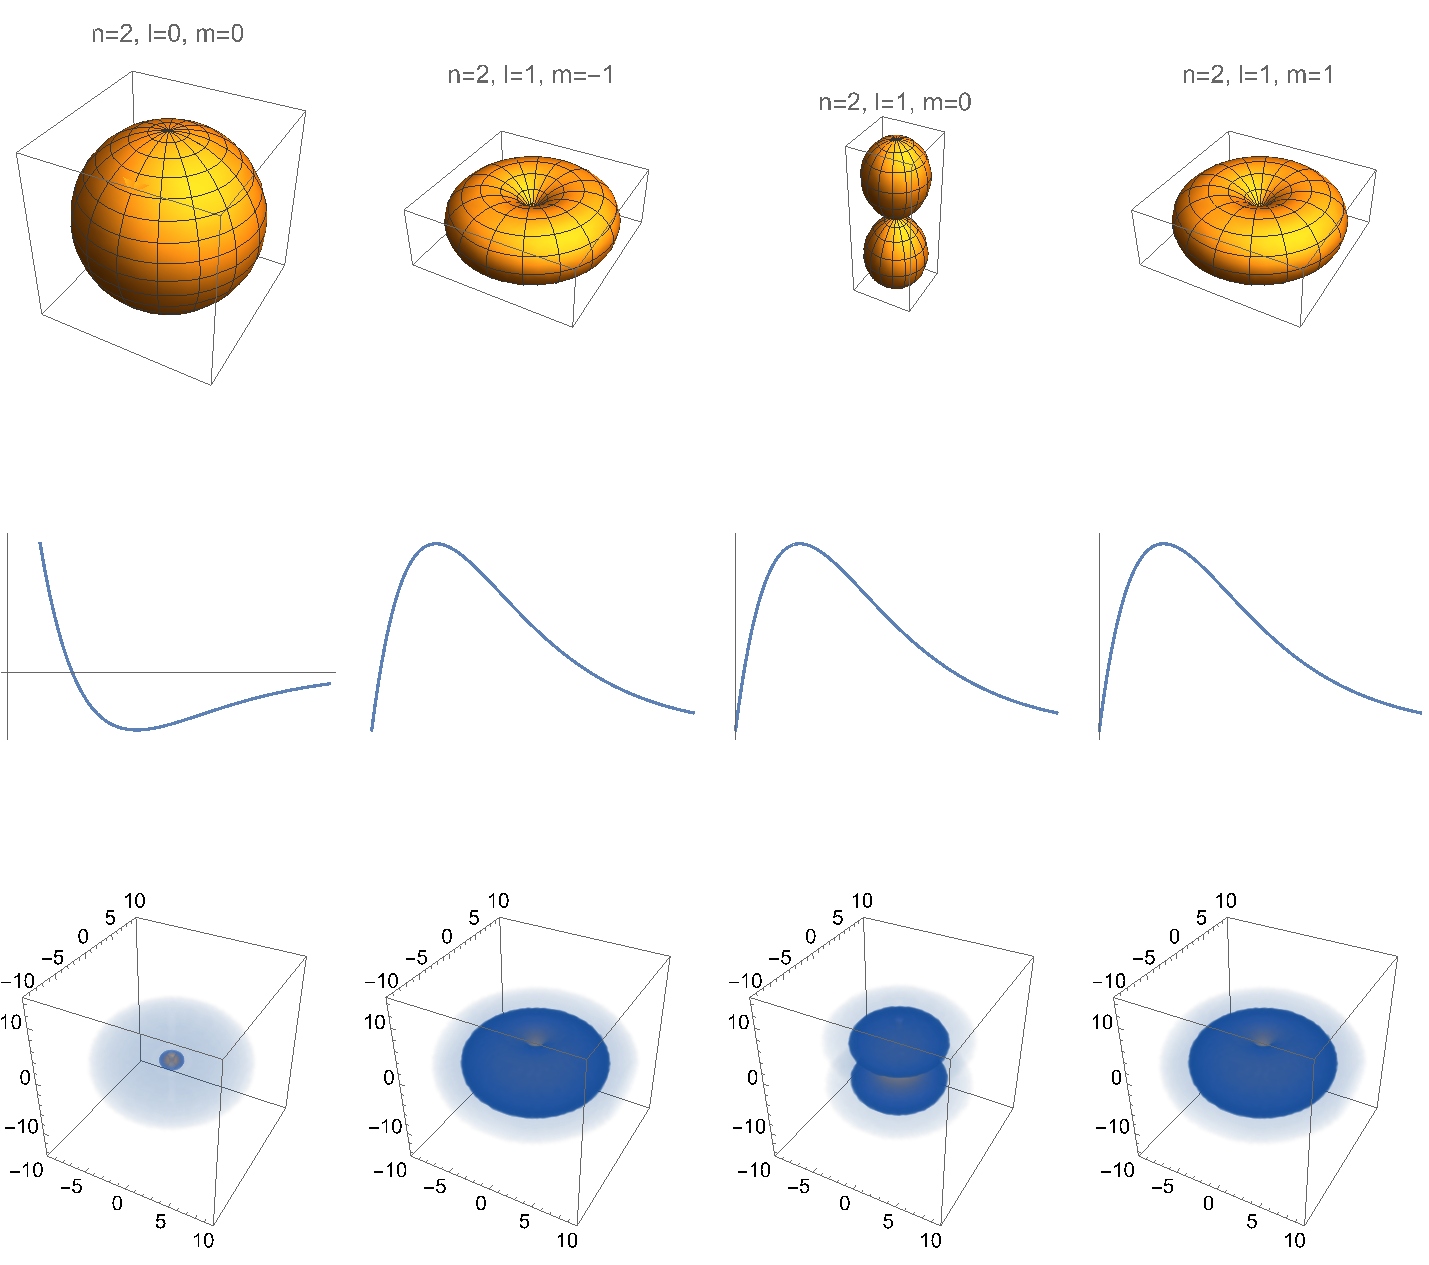
\includegraphics[scale=0.85]{Orbitals}
		\end{minipage}
		On top you can see the spherical and radial probability of an electron in a hydrogen Atom for different Quantum numbers. Below is a density plot of the square modulus of the whole wave function (as product of the upper 2 plots). If you sum all 4 states up you can kind of recognize a radial symmetry, as the \( l=0, m=0 \) state is already symmetric and the other three apparently add up to a sphere. 
	\tcbline
		\item \(  \)
		\begin{flalign*}
			\langle \hat{r} \rangle &= \uint[V]{r\abs{\psi_{2,1,1}}^2}{V} = \uint[0,2\pi]{\uint[0,\pi]{\uint[0,\infty]{\frac{1}{24a_0^5}\expo[-][r/a]r^2 \frac{3}{8\pi}\sin(\theta)^2r r^2\sin(\theta)}{r}}{\theta}}{\phi} = &&\\
			&= \frac{1}{32a_0^5} \uint[0,\infty]{r^5\expo[-][r/a_0]}{r} \uint[0,\pi]{\sin(\theta)^3}{\theta} = \frac{1}{32a_0^5}\ 120a_0^6\ \frac{4}{3} = \dl{5a_0} &&\\[1em]
%			
			\langle \hat{r}^2 \rangle &= \uint[V]{r^2\abs{\psi_{2,1,1}}^2}{V} = \frac{1}{32a_0^5} \uint[0,\infty]{r^6\expo[-][r/a_0]}{r} \uint[0,\pi]{\sin(\theta)^3}{\theta} = \dl{30a_0^2} &&\\[1em]
%			
			\langle \Delta\hat{r}^2 \rangle &= \langle \hat{r}^2 \rangle - \langle \hat{r} \rangle^2 = 30a_0^2 - 25a_0^2 = \dl{5a_0^2} &&
		\end{flalign*}
	
		Bohrs model states that \( r_n = \tfrac{n^2}{Z}a_o \) so in the case of a hydrogen atom with \( Z = 1 \) and an electron described by \( \psi_{2,1,1} \) the model predicts a radius of \( r_2 = 4a_0 \).\\
		Considering (the probabilistic nature of) quantum mechanics one gets a radius of \( r_2 = 5a_0 \), which clearly contradicts Bohrs model.
	\tcbline
		\item \( d = 1.75 \unit{fm} \)
		\begin{flalign*}
			P &= \uint[V]{\abs{\psi_{2,0,0}}^2}{V} = \uint[0,2\pi]{\uint[0,\pi]{\uint[0,d]{\frac{1}{4a_0^3}\expo[-][r/a] \left(1-\frac{r}{a_0} + \frac{r^2}{4a_0^2}\right) \frac{1}{4\pi} r^2\sin(\theta)}{r}}{\theta}}{\phi} = &&\\
			&= \frac{1}{2a_0^3} \uint[0,d]{\expo[-][r/a] \left(1-\frac{r}{a_0} + \frac{r^2}{4a_0^2}\right) r^2}{r} = \dl{6.11 \times 10^{-15}} &&
		\end{flalign*}
	\end{enumerate}
\end{mybox}

\begin{mybox}{Drehimpulsquantenzahlen}
	\centering \(  \)
	\tcblower
	\begin{enumerate}
		\item \( \hat{L}_z = -\iu\hbar\pdv{}{\phi};\quad \psi_{n,l,m} = a_m R_{n,l} \cos(\theta)\expo[\iu m\phi]P_l^m \)
		\begin{flalign*}
			\langle \hat{L}_z \rangle &= \uint[V]{\psi^* \hat{L}_z \psi}{V} = -\iu\hbar \uint[V]{\psi^* \pdv{\psi}{\phi}}{V} = \hbar m \uint[V]{\psi^* \psi}{V} = \dl{\hbar m} &&
		\end{flalign*}
	\tcbline
		\item \( \hat{\mathbf{L}}^2Y_l^m(\theta, \phi) = l(l+1)\hbar^2 Y_l^m (\theta, \phi) \)
		\begin{flalign*}
			\langle \hat{\mathbf{L}}^2 \rangle &= \uint[V]{\psi^* \hat{\mathbf{L}}^2 \psi}{V} = \uint[V]{\psi^* R_{n,l} \hat{\mathbf{L}}^2 Y_l^m}{V} = l(l+1)\hbar^2 \uint[V]{\psi^* \psi}{V} = \dl{l(l+1)\hbar^2} &&
		\end{flalign*}
	\tcbline
		\item \(  \)
		\begin{flalign*}
			\left[\hat{\mathbf{L}}^2, \hat{L}_z \right]\psi_{n,l,m} &= \hat{\mathbf{L}}^2 (\hat{L}_z \psi_{n,l,m}) - \hat{L}_z (\hat{\mathbf{L}}^2 \psi_{n,l,m}) = &&\\
			&= \hat{\mathbf{L}}^2 \hbar m\psi_{n,l,m} - \hat{L}_z l(l+1)\hbar^2 \psi_{n,l,m} = &&\\
			&= l(l+1)\hbar^3m \psi_{n,l,m} - l(l+1)\hbar^3m \psi_{n,l,m} = 0 &&
		\end{flalign*}
	\end{enumerate}
\end{mybox}

\begin{mybox}{Zeeman–Effekt}
	\centering \(  \)
	\tcblower
	\begin{enumerate}
		\item \(  \)
		\begin{flalign*}
			E &= V + T = \dl{-\vec{\mu} \cdot \vec{B} + \tfrac{1}{2}m(\dvec{r})^2} &&
		\end{flalign*}
	\tcbline
%		\item From a classical point of view, the electron is circulating around the nucleus. This moving charge can be viewed as a current in a closed loop, which in the presence of a magnetic field has a magnetic moment associated with it. The electron however does not move towards the nucleus due to its angular momentum. From a classical perspective the angular momentum prevents the electron from moving towards the proton and is therefore proportional to the magnetic moment.\\
		\item 
		\( \vec{B} = B\vec{e}_z;\quad |L_z| = \hbar m;\quad \vec{p}_{\text{m}} = -\tfrac{e}{2m_e}\vec{L} \)
		\begin{flalign*}
			E_{\text{pot, B}} &= -\vec{p}_{\text{m}} \cdot \vec{B} = \tfrac{e}{2m_e} \vec{L} \cdot \vec{B} = \tfrac{e\hbar}{2m_e}mB &&\\
			E_{n,l,m} &= E_{n,l}  + \tfrac{e\hbar}{2m_e}mB &&\\
			\Delta E &= \dl{\tfrac{e\hbar}{2m_e}mB} &&
		\end{flalign*}
	\tcbline
		\item 
		\begin{tikzpicture}
			\coordinate (O) at (-2,0) {};
			\coordinate (N) at (1,0) {};
			\foreach \i [count=\xi] in {-2,...,2}{
				\tkzDefPoint(1.5, \i){L\xi}
				\tkzDefPoint(2.5, \i){M\xi}
				\draw [dashed, line width=1pt] (N) -- (L\xi);
				\draw [line width=1pt] (L\xi) -- (M\xi) node [right] {\( m = \i \)};}
			
			\draw [line width=1pt] (O) -- (N) node [above, pos=0.5] {\( n=3, l=2 \)}; 
			
			\begin{scope}[shift={(7, 0)}]
				\coordinate (O) at (-2,0) {};
				\coordinate (N) at (1,0) {};
				\foreach \i [count=\xi] in {-1,...,1}{
					\tkzDefPoint(1.5, \i){L\xi}
					\tkzDefPoint(2.5, \i){M\xi}
					\draw [dashed, line width=1pt] (N) -- (L\xi);
					\draw [line width=1pt] (L\xi) -- (M\xi) node [right] {\( m = \i \)};}
				
				\draw [line width=1pt] (O) -- (N) node [above, pos=0.5] {\( n=2, l=1 \)}; 
			\end{scope}
		\end{tikzpicture}
	\tcbline
		\item \(  \)
		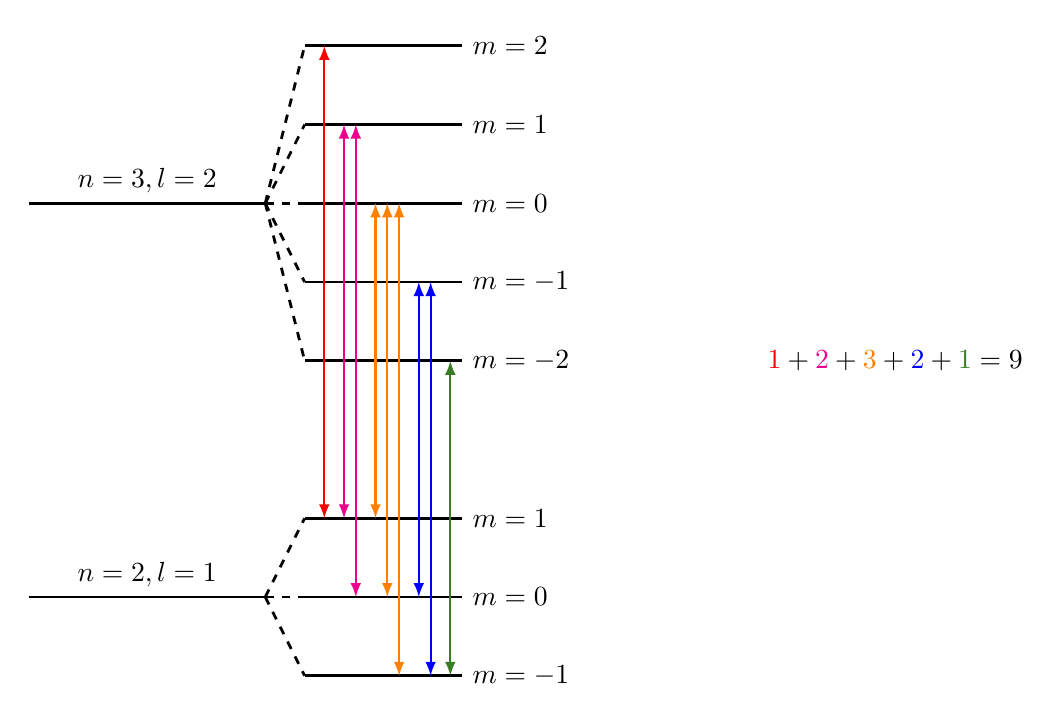
\begin{tikzpicture}
			\coordinate (O) at (-2,0) {};
			\coordinate (N) at (1,0) {};
			\foreach \i [count=\xi] in {-2,...,2}{
				\tkzDefPoint(1.5, \i){L\xi}
				\tkzDefPoint(3.5, \i){M\xi}
				\draw [dashed, line width=1pt] (N) -- (L\xi);
				\draw [line width=1pt] (L\xi) -- (M\xi) node [right] {\( m = \i \)};}
			
			\draw [line width=1pt] (O) -- (N) node [above, pos=0.5] {\( n=3, l=2 \)}; 
			
			\begin{scope}[shift={(0, -5)}]
				\coordinate (O) at (-2,0) {};
				\coordinate (N) at (1,0) {};
				\foreach \i [count=\xi] in {-1,...,1}{
					\tkzDefPoint(1.5, \i){L\xi}
					\tkzDefPoint(3.5, \i){M\xi}
					\draw [dashed, line width=1pt] (N) -- (L\xi);
					\draw [line width=1pt] (L\xi) -- (M\xi) node [right] {\( m = \i \)};}
				
				\draw [line width=1pt] (O) -- (N) node [above, pos=0.5] {\( n=2, l=1 \)}; 
			\end{scope}
		
			\foreach \i\j\k\l [count=\xi] in {2/1/red/0, 1/1/magenta/0.1, 1/0/magenta/0.1, 0/1/orange/0.2, 0/0/orange/0.2, 0/-1/orange/0.2, -1/0/blue/0.3, -1/-1/blue/0.3, -2/-1/OliveGreen/0.4}{
				\draw[line width=0.75pt, \k, latex-latex] (1.6+\xi*0.15+\l, \i) -- (1.6+\xi*0.15+\l, \j - 5);}
			
			\node at (9, -2) {\( \textcolor{red}{1} + \textcolor{magenta}{2} + \textcolor{orange}{3} + \textcolor{blue}{2} + \textcolor{OliveGreen}{1} = \dl{9} \)};
		\end{tikzpicture}
	\end{enumerate}
\end{mybox}

\end{document}